


\setcounter{mtc}{3}
\chapter{ Présentation du protocole de Certification FSSC 22 000 version 5}
\minitoc %insert la minitoc
\graphicspath{{Chapter1/figures/}}

%\DoPToC

%==============================================================================
\pagestyle{fancy}
\fancyhf{}
\fancyhead[R]{\bfseries\rightmark}
\fancyfoot[R]{\thepage}
\renewcommand{\headrulewidth}{0.5pt}
\renewcommand{\footrulewidth}{0pt}
\renewcommand{\chaptermark}[1]{\markboth{\MakeUppercase{\chaptername~\thechapter. #1 }}{}}
\renewcommand{\sectionmark}[1]{\markright{\thechapter.\thesection~ #1}}

\begin{spacing}{1.2}
%==============================================================================
\section*{Introduction}
Dans ce chapitre on va introduire avec un bref historique concernant les  normes de sécurité alimentaire pour ensuite présenter le protocole de certification FSSC 22 000 version 5, ses constituants ainsi que les principaux changements de la dernière version de la norme ISO 22000

\section{Les normes de sécurité alimentaire}
Au fil des ans, de nombreuses normes de sécurité alimentaire ont évoluée en vue de renforcer la sécurité alimentaire et d'aborder les questions soulevées par les fabricants, fournisseurs, détaillants et consommateurs:

\begin{itemize}
 \item \textbf{1938:} Application des Pratiques de bonne fabrication pour les aliments, médicaments et cosmétiques
  \item \textbf{1960:} Création des principes d’ HACCP
	 \item \textbf{1998:} Introduction de la norme First British Retail Consortium (BRC)
	  \item \textbf{Fin 1990:} Lancement de GlobalGAP ( bonnes pratiques agricoles)
		 \item \textbf{Mai 2000:} Création du GFSI.( évaluer les performances des programmes de management de sécurité alimentaire en vue de la convergence entre normes de sécurité alimentaire. )
		  \item \textbf{1995:} Lancement de la norme de Qualité et Sécurité Alimentaire (SQF)
			 \item \textbf{2004:} Lancement de la Norme Alimentaire Internationale (IFS)
			  \item \textbf{2005:} Emission de la norme ISO 22000:2005,( non approuvée par GFSI en raison du manque de programmes préalables suffisants. )
				 \item \textbf{2008:} Emission de PAS 220:2008 comme moyen de créer des programmes préalables suffisants pour ISO 22000:2005.
				  \item \textbf{2009:} Émission de FSSC 22000 (combinaison d’ISO 22000:2005 et de PAS 220:2008.
					 \item \textbf{Fév 2010:} Approbation du Contenu de FSSC 22000 par le GFSI
\end{itemize}
\section{FSSC 22000: Food Safety System Certification 22000}
\subsection*{Introduction}
Le référentiel FSSC 22000 (Food Safety System Certification 22000) est le dernier standard de certification  pour les fabricants de produits alimentaires. Il a été développé par la Fondation pour la certification en matière de sécurité alimentaire (Foundation for Food Safety Certification) et a été entièrement approuvé par le Global Food Safety Initiative (GFSI).


La FSSC 22000 est une combinaison de :
\begin{itemize}
	\item \textbf{ISO 22000:} Systèmes de management de la sécurité des denrées alimentaires-exigences pour tout organisme appartenant à la chaîne alimentaire.
	\item \textbf{ISO/TS 22002-1:} Programmes prérequis pour la sécurité des denrées alimentaires, partie 1 : fabrication des denrées alimentaires.
	\item \textbf{Exigences additionnelles FSSC 22 000:} Exigences supplémentaire FSSC 22 000 pour fournir la cohérence, l’intégrité et assurer la gouvernance et la gestion du système.
\end{itemize}

\subsection{Avantages de FSSC 22000}
FSSC 22000 est la norme des systèmes de gestion de sécurité alimentaire la plus exhaustive car, elle :


\begin{itemize}
	\item Est compatible et s'intègre facilement avec d’autres systèmes de gestion
	\item Incorpore totalement les Programmes préalables , ISO 22000:2018, ISO/TS  22002-1:2009 ,HACCP
	\item Évalue les risques réels relatifs à ses produits vis à vis de ses clients et consommateurs
	\item Instaure une organisation efficace d’identification, surveillance et maîtrise des risques sanitaires auxquels seront confrontés ses denrées alimentaires.
	\item Structure un outil d’amélioration de la performance en matière de sécurité des aliments et les moyens de surveiller efficacement cette performance.
	\item Promeut la conformité légale
	\item Accroît la transparence dans toute la chaîne logistique alimentaire
	\item Elle incorpore de nombreux principes d’autres normes alimentaires
      approuvées par la GFSI et les combine dans une approche unique.
\end{itemize}
\subsection{La norme ISO 22000}
L’ISO 22000  représente un référentiel standard ayant une portée internationale. Sa genèse était sous l’initiative du Danemark, qui a déposé en 2000 à travers  l’association danoise de normalisation sa proposition de norme internationale au comité technique de l’ISO. En 2001, le comité technique de l’ISO accepte la proposition, et constitue un groupe de travail animé par les danois. Les travaux ont duré 3 ans en collaboration avec les 45 pays les plus influents dans le commerce international des produits alimentaires. C’est ainsi que naît la première version de la norme ISO 22000 publiée pour la première fois en octobre 2005. Le 19 juin 2018, l’ISO a publié la nouvelle version de la norme ISO 22000
\subsubsection{Naissance de l’ISO 22000}

\subsubsection{Les changements sur la forme de la norme ISO 22 000: 2018}

\subsubsection{Nouvelle structure  HLS (High Level Structure )}
\paragraph{Définition}

C’est une structure unifiée et convenue avec un texte de base identique et des termes et définitions de base communs . La structure cadre comprend les articles principaux (1 à 10) et leur titre, selon une séquence établie : Les 3 premiers articles sont relativement généraux et ne contiennent pas d’exigences, Les 7 suivants peuvent être regroupés selon le modèle PDCA ( figure 3)

\begin{figure}[!ht]\centering
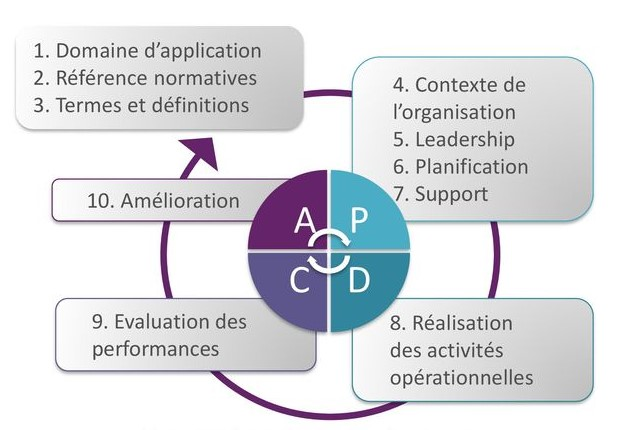
\includegraphics[scale=2.5]{image7.jpg}
\caption{Structure cadre universelle de la norme}
\label{fig:fig1}
\end{figure}

\paragraph{Intérêt}

La structure HLS  permet l’alignement de toutes les normes ISO de systèmes de management et l’amélioration de leurs compatibilités. Cette approche est utile pour les organismes qui choisissent de mettre en œuvre un système de management unique ( « intégré ») permettant de satisfaire simultanément aux exigences de deux normes de systèmes de management ou plus.

\subsubsection{Approche processus et cycle PDCA}

Pour atteindre les résultats escomptés conformément à la politique de sécurité des denrées alimentaires et à l’orientation stratégique de l’organisme , ce dernier  doit contribuer à son efficacité et efficience en adoptant une approche processus qui permet de comprendre et piloter les processus en interaction comme un système. L’approche processus doit s’appuyer sur une identification systématique et un management des processus.Elle comprend également un travail sur les interactions entre processus [3].  Selon la norme, le management des processus et du système dans son ensemble peut être réalisé en appliquant le cycle PDCA. Le PDCA est le principe de l’amélioration continue selon la  roue de Deming (figure 4) :
\begin{itemize}
	\item P (Plan) : prévoir, planifier, spécifier, définir
	\item D (Do) : faire, mettre en œuvre (en maîtrisant)
	\item C (Check) : vérifier, évaluer
	\item A (Act) : réagir, agir, améliorer.
\end{itemize}

\begin{figure}[!ht]\centering
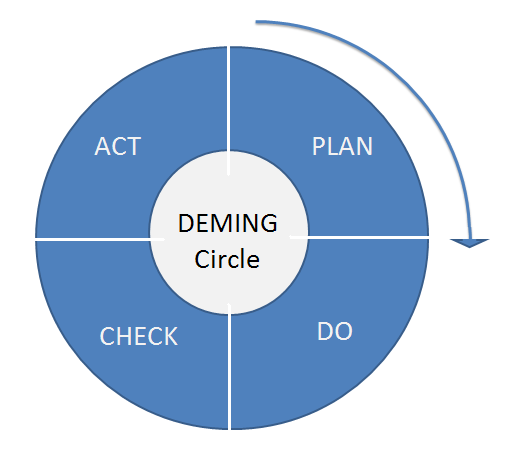
\includegraphics[scale=0.3]{image2.png}
\caption{Roue de Deming (cycle PDCA)}
\label{fig:fig1}
\end{figure}


Dans la norme ISO 22000:2018 , l’approche processus utilise le cycle PDCA à deux niveaux distincts, opérant l’un dans l’autre. L’un couvre le cadre global du SMSDA ( chapitres 4 à 7, 9 et 10 de la norme). L’autre concerne la réalisation des activités opérationnelles couvrant simultanément les principes HACCP ( chapitre 8). Cela signifie que la communication entre les deux niveaux est essentielle. (Figure 5)


\begin{figure}[!ht]\centering
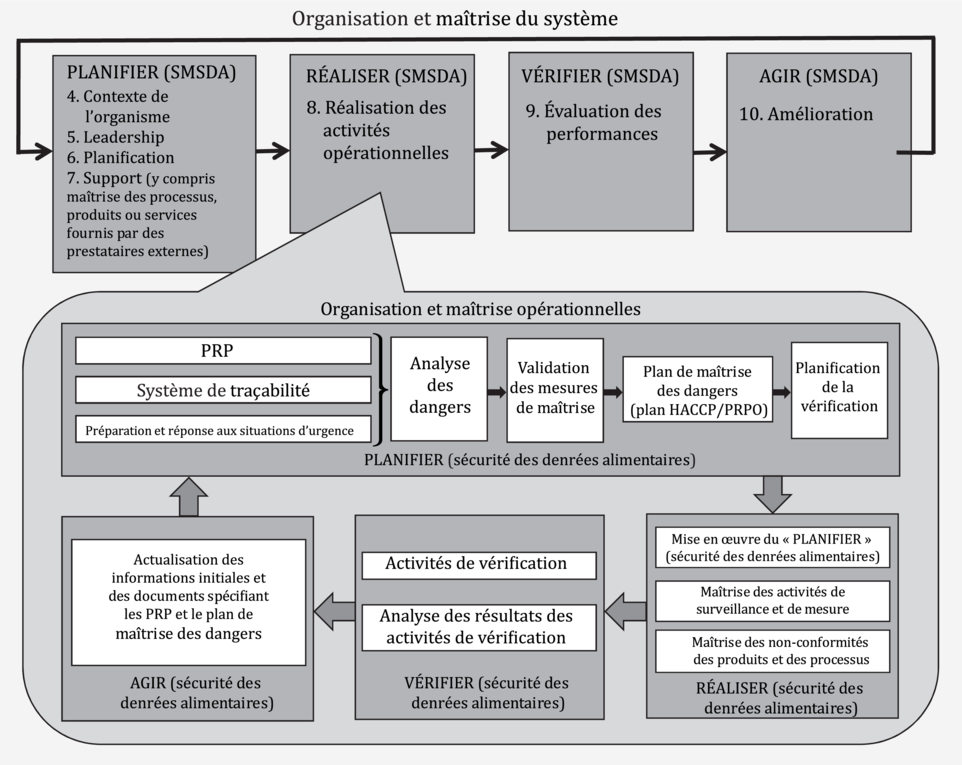
\includegraphics[scale=5]{image1.png}
\caption{ Illustration des deux cycles PDCA [3]}
\label{fig:fig1}
\end{figure}

\subsubsection{Modifications au niveau de la terminologie}
la « responsabilité de la direction » devient le « leadership ». La politique et les objectifs doivent être compatibles avec le contexte de l’organisme (enjeux internes et externes) et avec les exigences des parties intéressées pertinentes. Les exigences liées au système de management doivent être intégrées aux processus métiers. Par ailleurs, la direction doit orienter et soutenir les personnes pour qu’elles contribuent à l’efficacité du système ;




le « management des ressources » devient le « support ». Alors qu’il s’agissait dans la version 2005 de gérer les ressources mises à disposition de manière un peu statique, la notion de support indique une note plus dynamique de soutien, incluant les acteurs en support à plus d’engagement dans la contribution à la sécurité du produit et des services ;





les « documents et enregistrements » tels que les procédures, modes opératoires, instructions deviennent les « informations documentées » ;




la « planification et réalisation de produits sûrs » devient la « réalisation des activités opérationnelles ». Cette nouvelle terminologie permet de prendre en compte des activités à caractère opérationnel proches de la production en intégrant la chaîne logistique étendue ;






le « produit » devient les « produit et service ». Le terme « produit » était générique dans la version 2005. Les activités de prestations de services, pourtant couvertes par la norme pouvaient se sentir moins concernées ou, tout du moins, trouver que l’ancienne terminologie avait une prégnance industrielle trop marquée ;





les « fournisseurs » deviennent les « prestataires externes ». Cela renforce le côté « prestation » de tout fournisseur, même lorsque celle-ci consiste à livrer des matières premières, des ingrédients ou des emballages, ou à les stocker.



\subsubsection{Nouveautés au niveau des définitions}
Les nouvelles définitions sont :


\begin{itemize}
	\item  le niveau acceptable : Ce terme était déjà utilisé dans la version 2005 sans jamais  avoir été défini
	\item  le critère d’action
	\item  la contamination
	\item  l’information documentée
	\item  l’aliment pour animaux producteurs de denrées alimentaires
	\item  une denrée alimentaire
	\item  l’aliment pour animaux non producteurs de denrées alimentaires
	\item  une partie intéressée (ou partie prenante)
	\item  un lot
	\item  une mesure
	\item  un objectif
	\item  l’organisme
	\item  l’externalisation
	\item  la performance
	\item  le risque
	\item  un danger significatif
	\item  la direction
	\item  la traçabilité
\end{itemize}



Les définitions modifiées sont :


\begin{itemize}
	\item  la mesure de maîtrise : La notion « éliminer un danger » a disparu.
	\item  le CCP (point critique pour la maîtrise) : la mesure doit être « à temps », ce qui implique l’absence de délai notable entre la déviation et sa détection.
	\item la surveillance
	\item  le programme prérequis opérationnel (PRPO)
	\item  le programme prérequis (PRP)
	\item  le produit
	\item  la validation : La définition est plus appropriée, dans le domaine de la sécurité des denrées alimentaires, que la définition contenue dans l’ISO 9001:2015.
\end{itemize}

\subsubsection{ La documentation }
Les exigences relatives à la documentation de l’article 4.2 de la version 2005 sont dans l’article 7.5[2] . Les documents (procédures, instructions, modes opératoires, standards de fabrication, fiches de bonnes pratiques, etc.) et les enregistrements (résultats des surveillances, des contrôles, mesures, traçabilité...) sont regroupés en tant qu’informations documentées. Avec cette version, l’organisme a le choix des supports pour les informations documentées. En effet, la norme n’impose plus de procédures systèmes. C’est à l’organisme de définir le niveau de « granulométrie » du système documentaire en fonction des risques et des compétences disponibles . On passe donc de la culture de la méthode à la culture du résultat.
\subsubsection{ Principaux changements sur le fond de la norme ISO 22000:2018 }

selon la norme ISO 22 000:2018  le leadership est au cœur  du  « mécanisme » d’amélioration induit par le système de management, à l’image d’une « pile » qui fournirait l’énergie pour mettre le concept du PDCA en mouvement.
Le système doit prendre en considération comme donnée d’entrée le contexte dans lequel il évolue, les exigences des clients, ainsi que les besoins et attentes des parties intéressées qui ont une incidence sur le système de management de la sécurité des denrées alimentaires et ses processus. En effet, un système de management ne peut développer sa pleine efficacité et atteindre ses résultats attendus que s’il est aligné avec le contexte et le fonctionnement de l’organisme.
Avec ces données d’entrée et de « l’énergie » impulsée par le leadership, le mécanisme d’amélioration s’exécute suivant l’approche processus, le cycle PDCA et l’approche risques/opportunités.


\begin{figure}[!ht]\centering
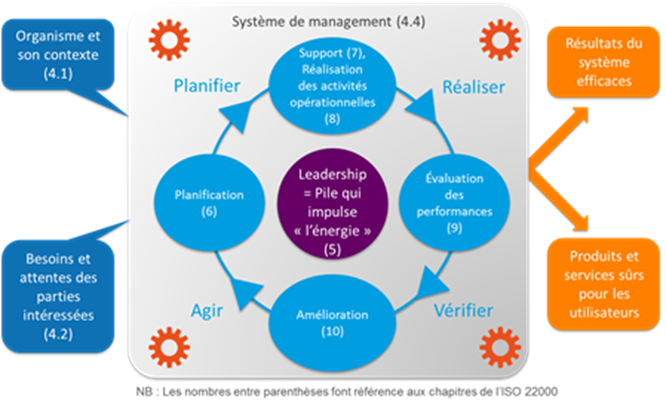
\includegraphics[scale=0.9]{image4.png}
\caption{ Représentation de la structure de la norme ISO 22000:2018 }
\label{fig:fig1}
\end{figure}

\subsubsection{Chapitre 4 de la norme -contexte de l’organisme }
Ce nouveau chapitre de la norme regroupe quatre exigences
\subsubsection{Compréhension de l’organisme et de son contexte ( PESTEL ou SWOT ) }
Cette nouvelle  exigence de la norme oblige l’organisme à s’intéresser à son contexte, en l’incitant à identifier ses enjeux internes et externes et à sélectionner ceux qui ont une influence avérée ou potentielle sur les résultats du système de management de la sécurité des denrées alimentaires  ce qui permet de relier  plus fortement la démarche de sécurité sanitaire des aliments à la « vraie vie » de l’organisme.
\subsubsection{Compréhension des besoins et attentes des parties intéressées}
La  version 2005 exigeait  une communication externe avec les parties intéressées [4] Cependant, la norme ISO 22000 :2018 exige  d’identifier, de revoir et d’actualiser les informations relatives aux parties intéressées dites « pertinentes »  et à leurs exigences(besoins et/ou attentes).Connaître les parties intéressées pertinentes, leur fonctionnement, leurs prises de positions et les relations qu’ils entretiennent entre eux vous permettra d’identifier plus facilement leurs préoccupations et de percevoir leur capacité de soutien (opportunités) ou d’opposition (risques).
\subsubsection{Système de management de la sécurité des denrées alimentaires et les processus associés }

Le processus se définit comme un ensemble d’activités corrélées ou en interaction qui transforme des éléments d’entrée en éléments de sortie avec la création d’une valeur ajoutée .
La norme ISO 22000:2018 exige d’établir, de mettre en œuvre, de maintenir, d’actualiser et d’améliorer en continu un système de management de la sécurité des denrées alimentaires, y compris les processus nécessaires et leurs interactions.[3]. Il existe des éléments nécessaires au pilotage d’un processus (Figure 7). Afin de décrire les interactions entre processus, il est possible d’utiliser le diagramme SIPOC. Au-delà de l’acronyme, c’est un outil de visualisation pour identifier tous les éléments pertinents associés à un processus : ses activités (P : Process), les sorties (O = Output), les entrées (I = Input), les fournisseurs (S = Suppliers) et les clients (C = Customers). Il est recommandé d’employer le SIPOC dans la phase initiale de description d’un processus (figure 13). ( partie pratique)

\begin{figure}[!ht]\centering
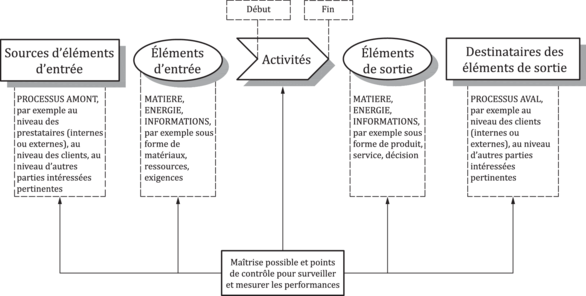
\includegraphics[scale=9]{image6.png}
\caption{ Représentation schématique des éléments d’un processus }
\label{fig:fig1}
\end{figure}


\subsubsection{Planification – Chapitre 6 de la norme}

C’est une nouvelle exigence qui impose la détermination des risques et des opportunités en lien avec les enjeux du contexte déterminés à l’article 4.1 et les besoins/attentes des parties intéressées retenues à l’article 4.2.

Il ne faut pas  confondre le mot risque définit comme étant << l’effet de l’incertitude sur les objectifs>> [6] avec le mot danger ou encore le risque au niveau de la sécurité sanitaire. En effet, l’article 6.1.1 de la norme mentionne que cela concerne les risques et les opportunités relatifs à l’atteinte des résultats visés du système de management de la sécurité des denrées alimentaires, dont ceux liés à la conformité des produits et services.
 Cet article encourage aussi bien la prévention et la réduction des effets négatifs (indésirables) que le développement des effets positifs (désirables).
La norme n’impose pas de méthode pour déterminer les risques et les opportunités mais il y a quelques notions élémentaires à connaître  permettant leur détermination et leur traitement :

\begin{itemize}
	\item l’événement qui est à l’origine du risque ou de l’opportunité
	\item sa vraisemblance qui est la probabilité d’occurrence de l’événement ;
\item sa conséquence qui est l’effet sur le produit, les processus ou le système
\item sa gravité ou son bénéfice qui est l’impact sur le produit, les processus ou le système.
\end{itemize}


L’article 6.1.2 prescrit des actions dans les processus du système de management de la sécurité des denrées alimentaires pour traiter les risques et les opportunités déterminés à l’article 6.1.1. 
%==============================================================================
\end{spacing}
